\documentclass{article}

\usepackage{amsthm, amsfonts, amsmath, amssymb}
\usepackage{graphicx}
\usepackage{fullpage}

\usepackage{xcolor}
\definecolor{commentsColor}{rgb}{0.497495, 0.497587, 0.497464}
\definecolor{keywordsColor}{rgb}{0.000000, 0.000000, 0.635294}
\definecolor{stringColor}{rgb}{0.558215, 0.000000, 0.135316}
\usepackage{listings}
\lstset{ %
	backgroundcolor=\color{white},   				% choose the background color; you must add \usepackage{color} or \usepackage{xcolor}
	basicstyle=\footnotesize\ttfamily,				% the size of the fonts that are used for the code
	breakatwhitespace=false,         				% sets if automatic breaks should only happen at whitespace
	breaklines=true,                 				% sets automatic line breaking
	captionpos=b,                    				% sets the caption-position to bottom
	commentstyle=\color{commentsColor}\textit,		% comment style
	frame=tb,	                   	   				% adds a frame around the code
	keywordstyle=\color{keywordsColor}\bfseries,	% keyword style
	language=Python,                 				% the language of the code (can be overrided per snippet)
	otherkeywords={*,...},           				% if you want to add more keywords to the set
	rulecolor=\color{black},         				% if not set, the frame-color may be changed on line-breaks within not-black text (e.g. comments (green here))
	stringstyle=\color{stringColor}, 				% string literal style
	title=\lstname,                  				% show the filename of files included with \lstinputlisting; also try caption instead of title
	columns=fixed                   				% Using fixed column width (for e.g. nice alignment)
}

\usepackage{hyperref}

\newtheorem{lemma}{Lemma}
\newtheorem{theorem}{Theorem}
\newtheorem{corollary}{Corollary}
\newtheorem{conjecture}{Conjecture}
\newtheorem{definition}{Definition}

\renewcommand{\O}{\mathcal{O}}

\begin{document}
	\title{A Better Chebyshev Algorithm}
	\author{William Boyles}
	\date{\today}
	\maketitle
	
	\section{Definitions}
	\begin{definition}
		$U(n,x)$ is the degree $n$ Chebyshev polynomial of the second kind and is defined by the following recurrence relation:
		\begin{equation*}
			U(n,x) = \begin{cases}
				1 & n = 0 \\
				2x & n = 1 \\
				2x U(n-1,x) - U(n-2,x) & n \geq 2
			\end{cases}.
		\end{equation*}
	\end{definition}
	\begin{definition}
		$f(n,x)$ is $U(x/2)$ over the field $GF(2)$.
		So, it is defined by the following recurrence relation where all operations happen mod 2:
		\begin{equation*}
			f(n,x) = \begin{cases}
				1 & n = 0 \\
				x & n = 1 \\
				x f(n-1,x) - f(n-2,x) & n \geq 2
			\end{cases}.
		\end{equation*}
	\end{definition}
	It's known that the nullity, $d(n)$ of an $n \times n$ \textit{Lights Out} board is the degree of $\gcd(f(n,x), f(n,1+x))$.
	So, one needs to be able to calculate $f(n,x)$ and $f(n,x+1)$ efficiently to calculate $d(n)$ efficiently.
	Ideally, the algorithm would not require calculating all of $f(0,x) \dots f(n-1,x)$ and $f(0,x+1) \dots f(n-1,x+1)$.
	We present such an algorithm which takes $\O(n)$ time and $\O(1)$ extra space.
	
	\section{Investigating Patterns}
	\subsection{Patterns in $f(n,x)$}
	Since $f(n,x)$ is a polynomial over $GF(2)$, all of its coefficients are either 1 or 0.
	So, a sensible way to visualize $f(n,x)$ would be to color squares black or white to represent the coefficients.
	For example,
	\begin{equation*}
		f(5,x) = 1x^5 + 0x^4 + 0x^3 + 0x^2 + 1x + 0 = \blacksquare\square\square\square\square\blacksquare\square.
	\end{equation*}
	If we plot out $f(0,x)$ through $f(128,x)$ in the same way, aligning terms of the same degree, we get the following image.
	
	\begin{center}
		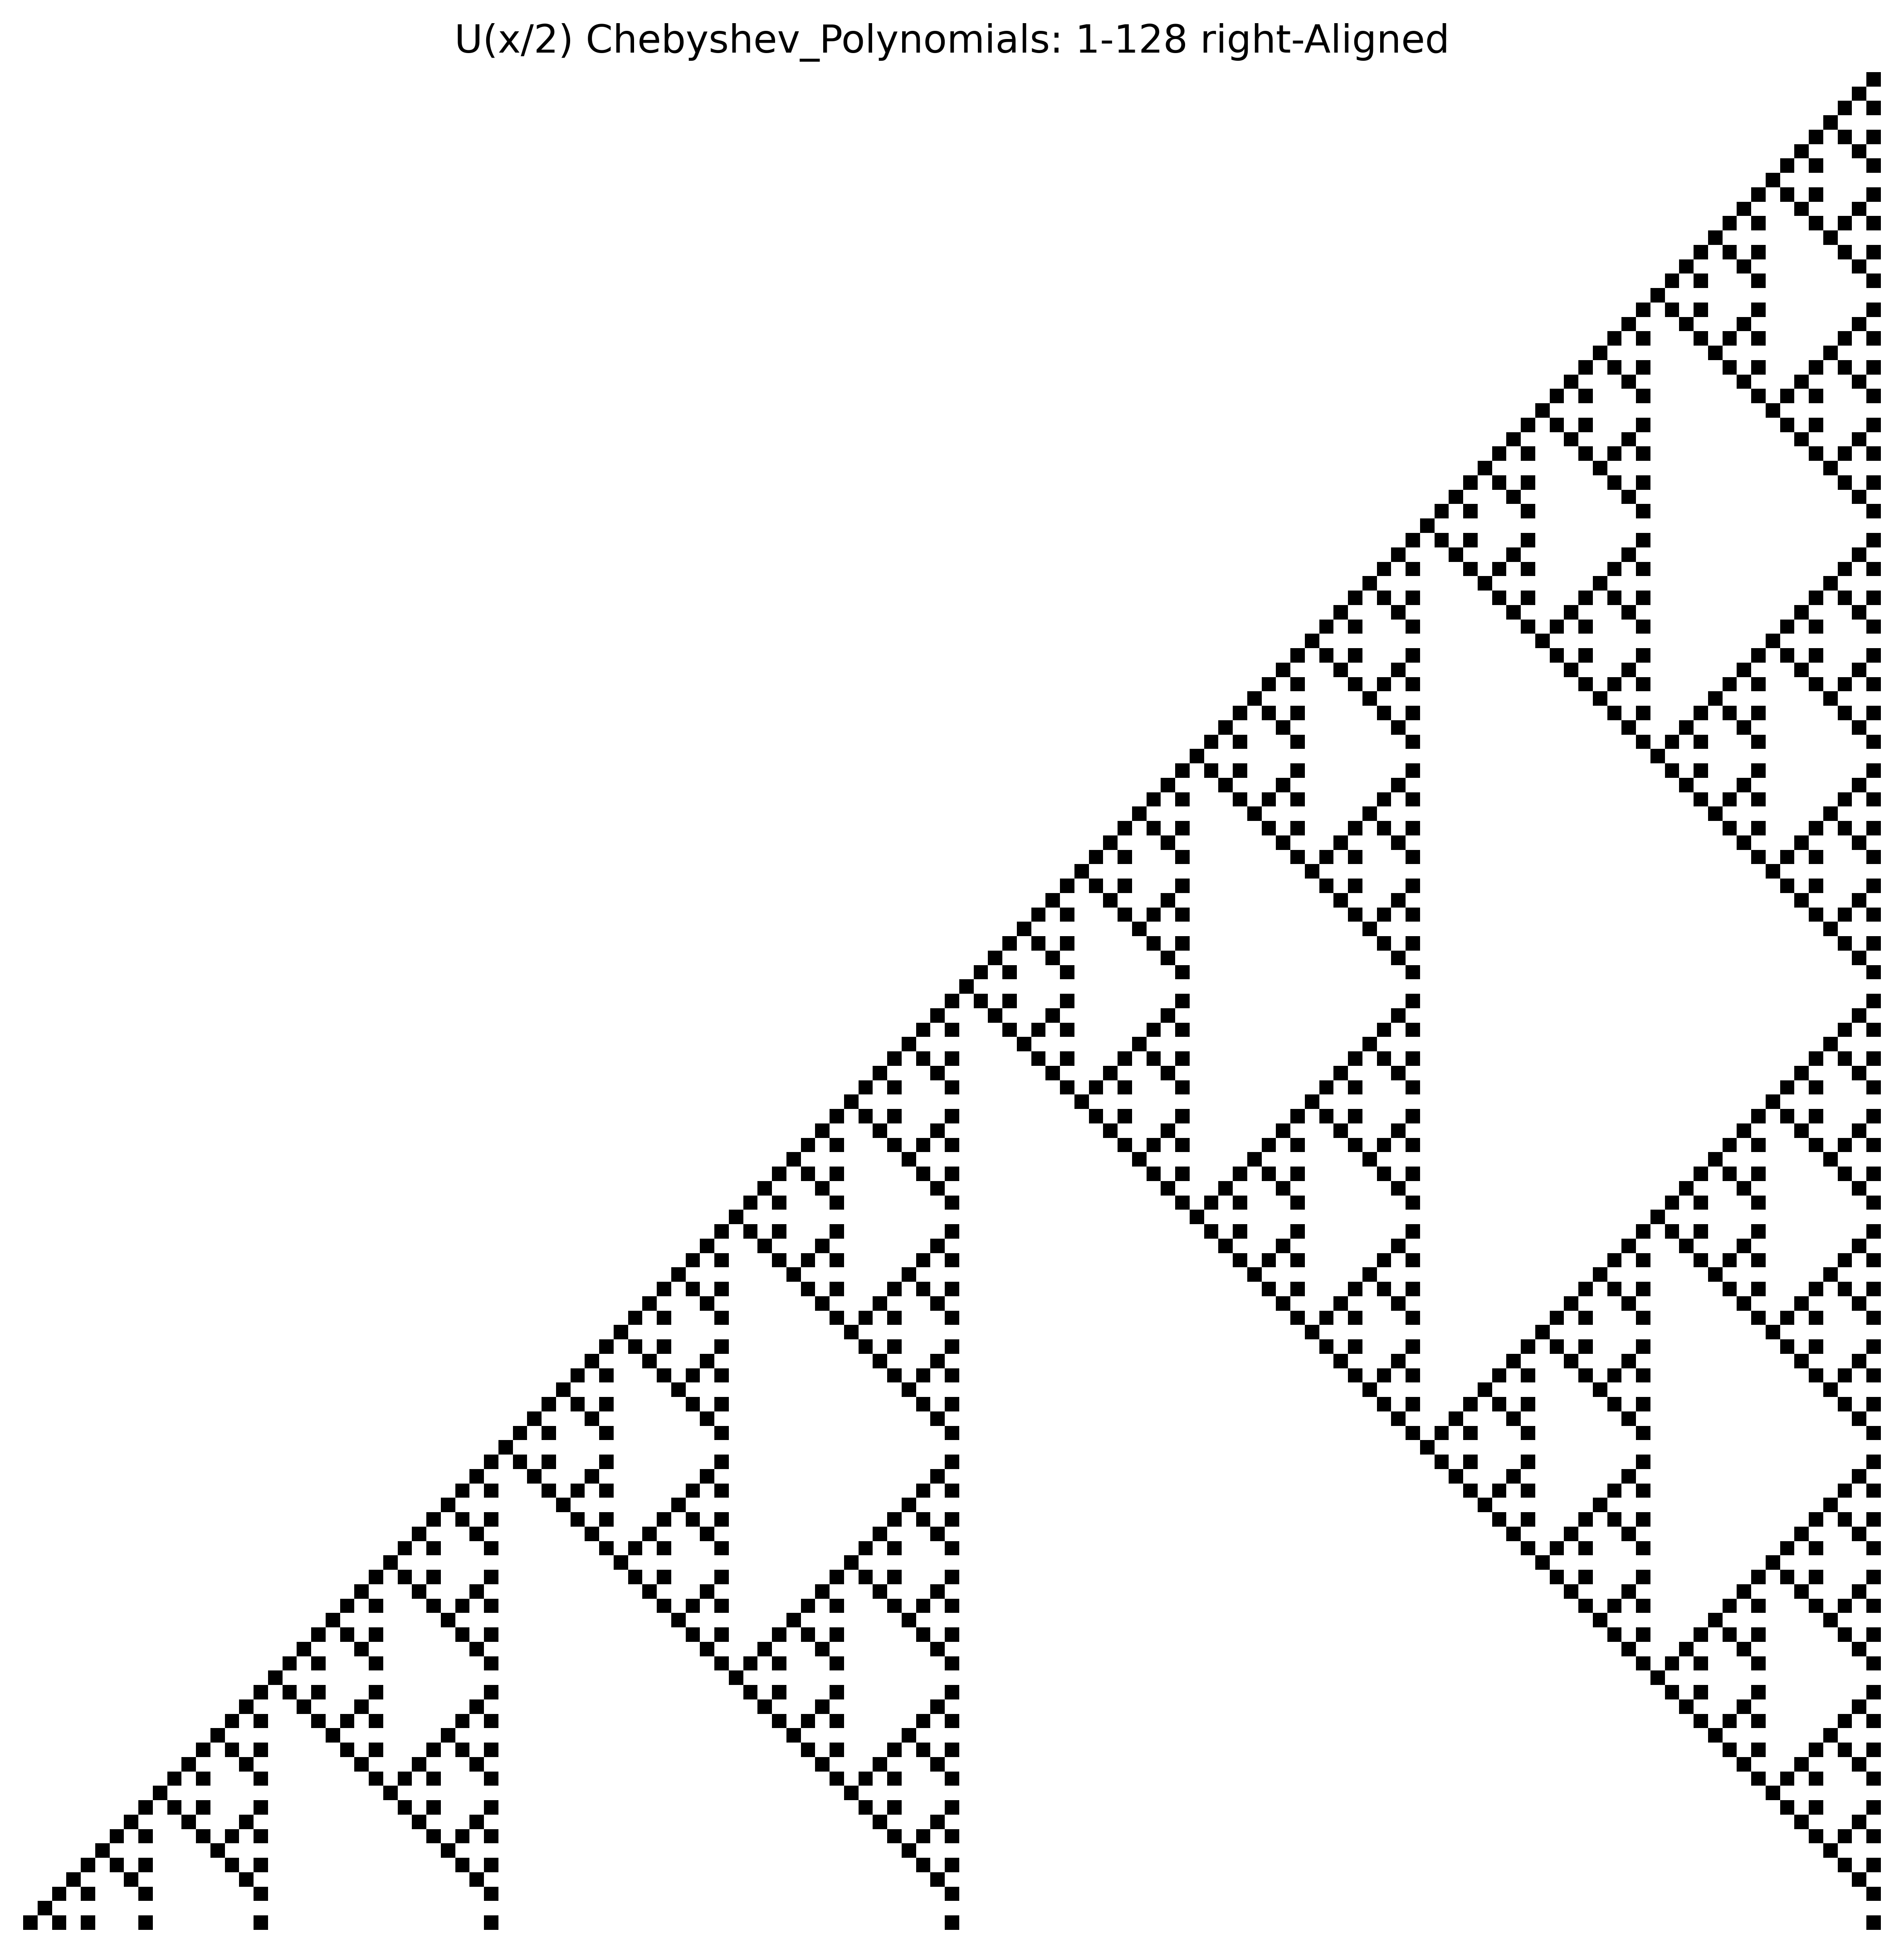
\includegraphics[width=.8\textwidth]{../../code/serialization/chebyshev/chebyshev1_right_128.png}	
	\end{center}

	This looks exactly like the right half of a Sierpinski Triangle rotated a counter-clockwise quarter-turn.
	However, the the length of each row in the Sierpinski Triangle grows by 1, and in our image, lengths grow by 2.
	So, we might suspect we are only seeing the even indexed rows of the triangle.
	It's well-known that the odd values of Pascal's Triangle form Sierpinski's Triangle.
	So, we might suspect that we can calculate coefficients of $f(n,x)$ by looking at the parity of binomial coefficients.
	
	\begin{conjecture}
		Let $f(n,x)_i$ be the $i$th entry in the coefficient list of $f(n,x)$ so that $f(n,x)_0$ is the highest degree term and $f(n,x)_n$ is the units term.
		Let $K = 2^k - 1$ where $k$ is the smallest integer such that $K \geq n$.
		Let $S = 2(K-n)$.
		Then
		\begin{equation*}
			f(n,x)_i = \begin{cases}
				1 & \binom{2i + S}{S + i} \text{ is odd} \\
				0 & \text{otherwise}
			\end{cases}.
		\end{equation*}
	\end{conjecture}

	Those familiar with cellular automaton might also recognize the above image as half of the symmetrical pattern formed by rule 90 with a starting condition of one black cell.

	\subsection{Parity of Binomial Coefficients}
	Here's a neat fact about the divisibility of binomial coefficients.
	\begin{theorem}[Kummer's Theorem]
		Let $p$ be a prime, $n$ and $m$ positive integers.
		Then the highest power of $p$ that divides $\binom{n+m}{m}$ is the number of carry operations when adding $n$ and $m$ in base $p$.
	\end{theorem}
	
	Since we're concerned with base 2, we can give a more specific version of this result.
	\begin{corollary}
		$\binom{n+m}{m}$ is odd if and only if the bitwise AND of $n$ and $m$, is 0.
	\end{corollary}
	This is an $\O(1)$ divisibility test, so we have an $\O(1)$ to calculate $f(n,x)_i$.
	
	
	\subsection{Patterns in $f(n,x+1)$}
	$f(n,x+1)$ is also a polynomial over $GF(2)$, so all of its coefficients are 1 or 0.
	So, we can visualize it in the same way we did for $f(n,x)$.
	For example,
	\begin{equation*}
		f(5,x+1) = 1x^5 + 1x^4 + 0x^3 + 0x^2 + 0x + 0 = \blacksquare\blacksquare\square\square\square\square.
	\end{equation*}
	Plotting $f(0,x+1)$ through $f(128,x+1)$ in the same way, aligning terms of the same degree, we get the following image.
	
	\begin{center}
		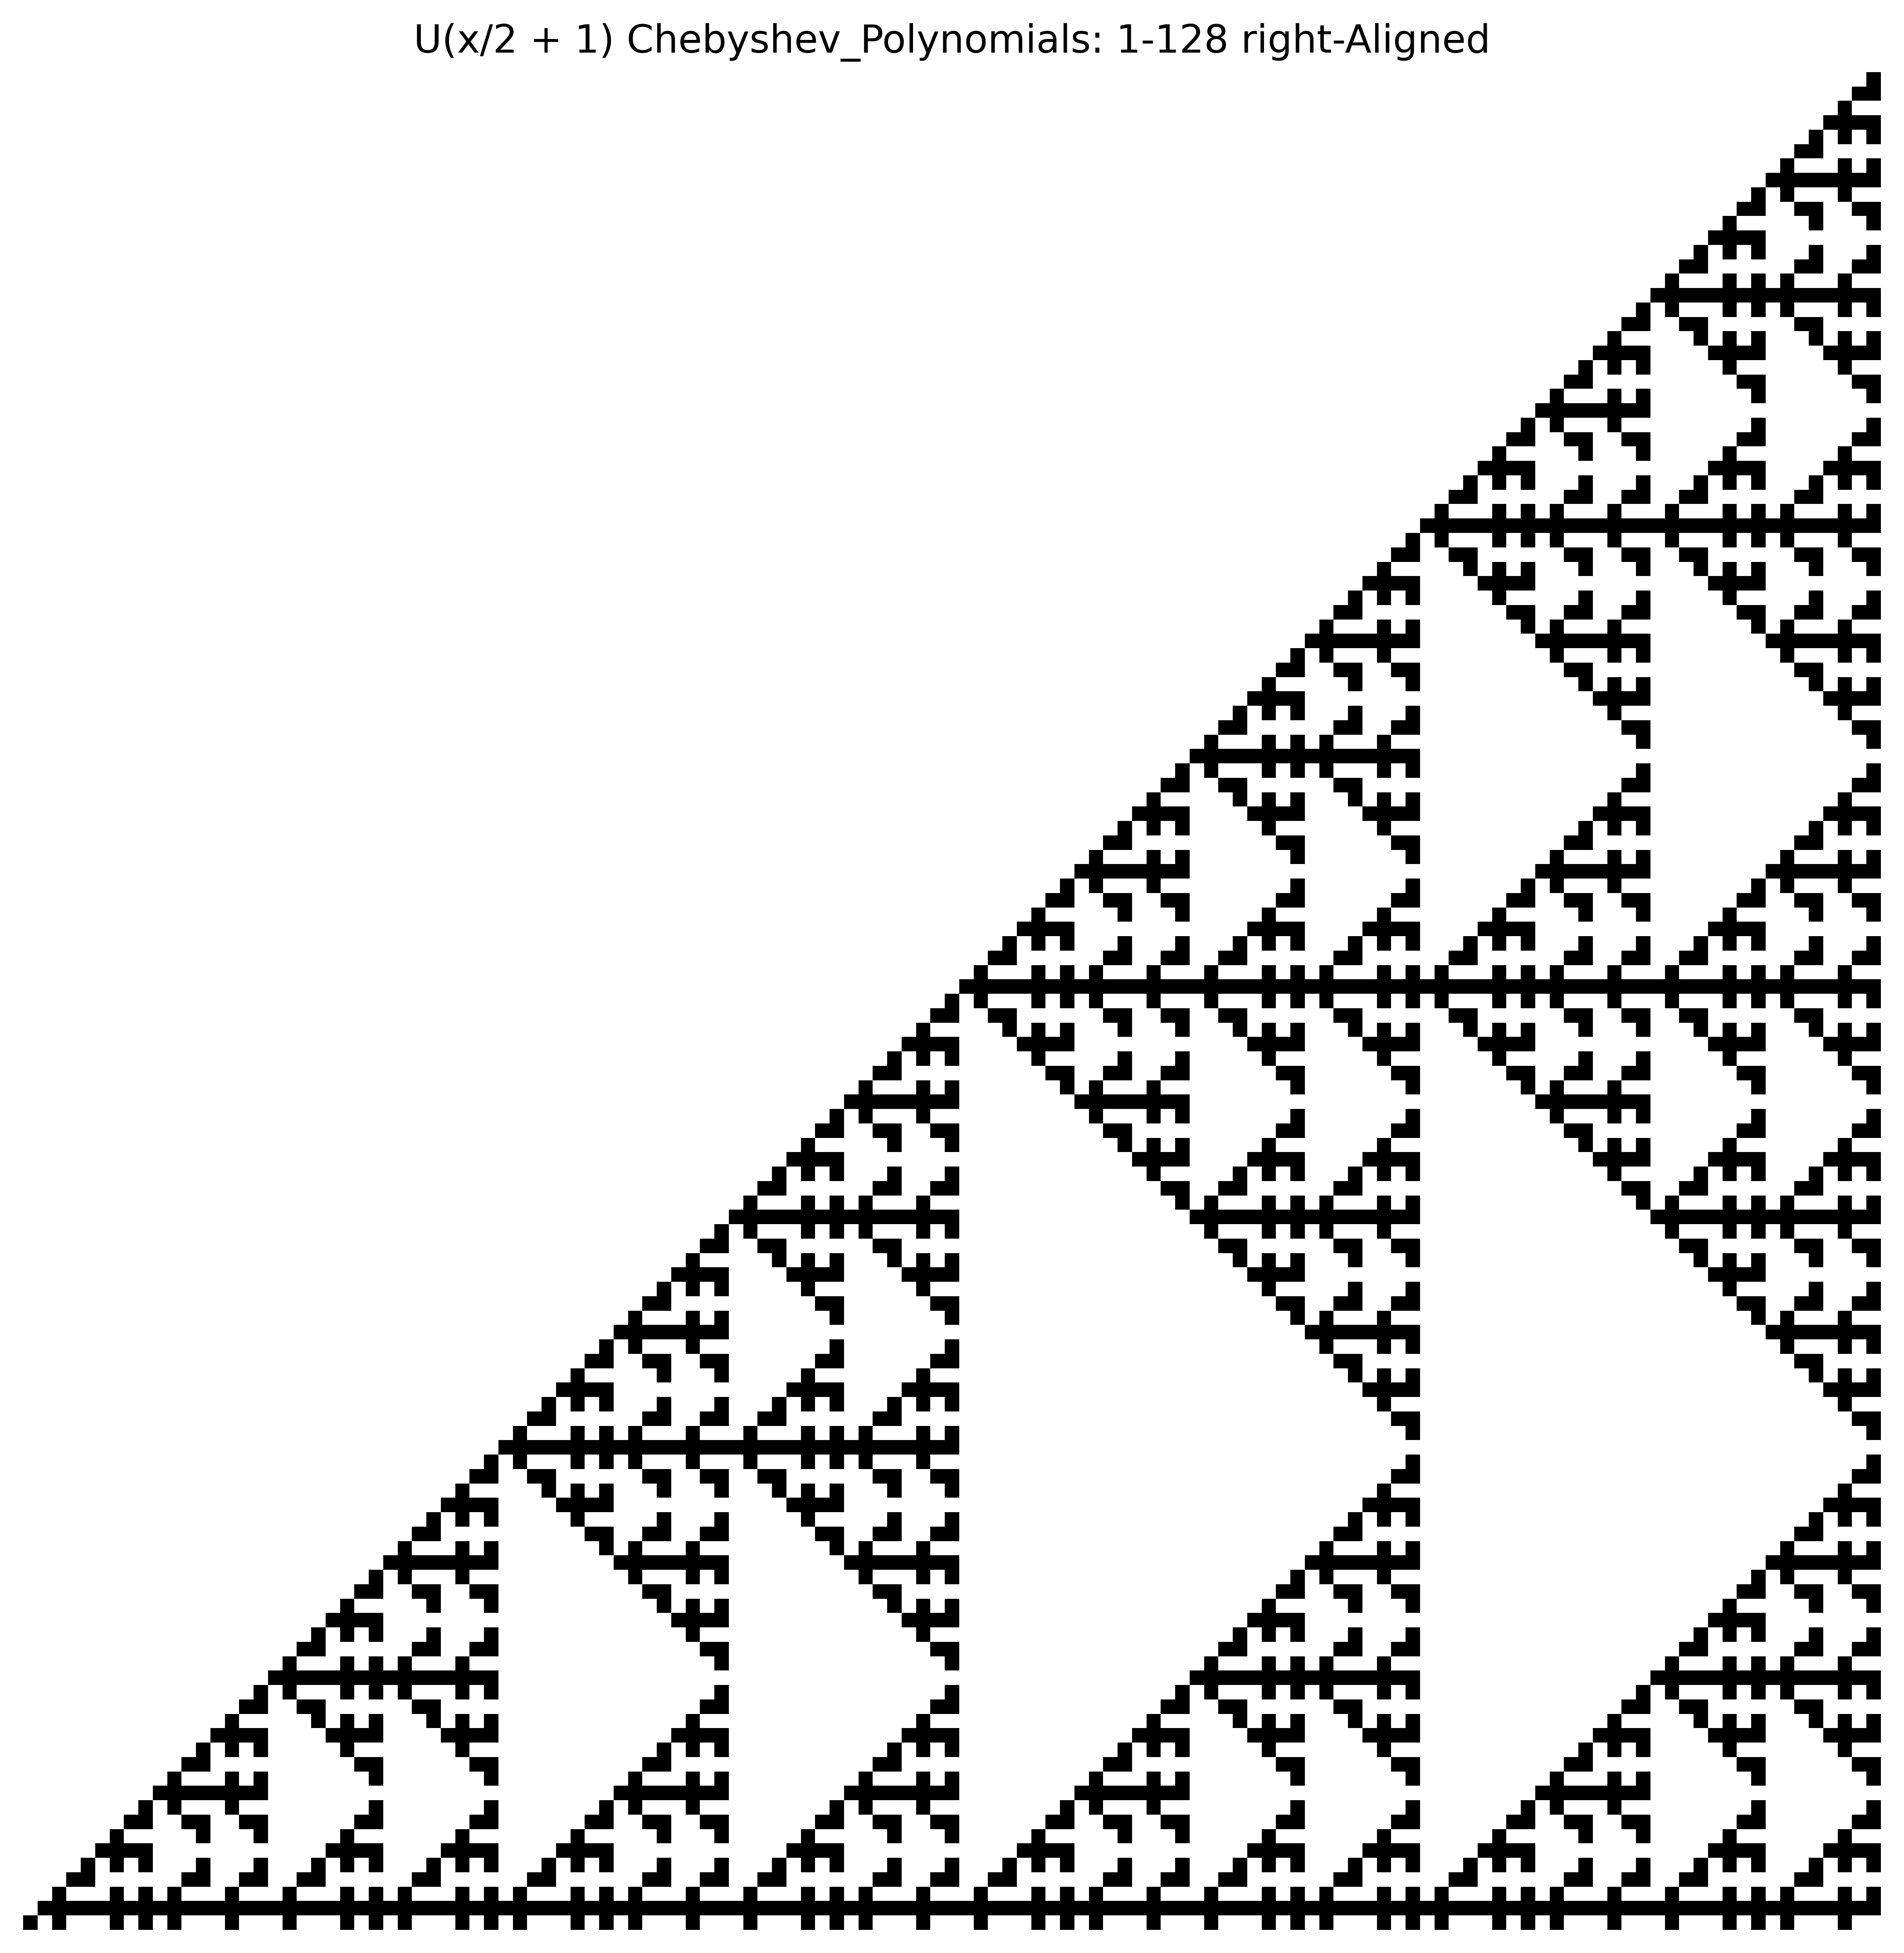
\includegraphics[width=.8\textwidth]{../../code/serialization/chebyshev/chebyshev2_right_128.png}	
	\end{center}

	Although perhaps not as familiar as the Sierpinski Triangle, this is easily recognizable to those familiar with cellular automaton as half of the symmetrical pattern formed by rule 150.
	Much like how one can obtain the pattern formed by rule 90 from odd numbers in the triangle of binomial coefficients (i.e. Pascal's Triangle), one can obtain the pattern formed by rule 150 from odd numbers in the triangle of trinomial coefficients known as the Trinomial Triangle, where each subsequent row has 2 more entries than the previous.
	
	\begin{definition}
		The trinomial coefficient in the $n$th row and $k$th column of the trinomial triangle, $\binom{n}{k}_2$ is defined by the following relationships:
		\begin{equation*}
			\binom{n}{k}_2 = \begin{cases}
				0 & k < 0 \text{ or } k > 2n + 1 \\
				0 & n < 0 \\
				1 & k = 0 \text{ and } n = 0 \\
 				\binom{n-1}{k-1}_2 + \binom{n-1}{k}_2 + \binom{n-1}{k+1}_2 & \text{otherwise}
			\end{cases}.
		\end{equation*}
	
		Equivalently, $\binom{n}{k}_2$ is the coefficient of the degree $k$ term in $(x^2 + x + 1)^n$.
	\end{definition}

	\begin{conjecture}
		Let $f(n,x+1)_i$ be the $i$th entry in the coefficient list of $f(n,x+1)$ so that $f(n,x+1)_0$ is the highest degree term and $f(n,x+1)_n$ is the units term.
		Let $K = 2^k - 1$ where $k$ is the smallest integer such that $K \geq n$.
		Let $S = K - n$.
		Then
		\begin{equation*}
			f(n,x+1)_i = \begin{cases}
				1 & \binom{S + i}{2S + i}_2 \text{ is odd} \\
				0 & \text{otherwise}
			\end{cases}.
		\end{equation*}
	\end{conjecture}
	
	
	\subsection{Parity of Trinomial Coefficients}
	Here's another fact similar to Kummer's Theorem about the divisibility of binomial coefficients.
	\begin{theorem}[Lucas's Theorem]
		Let $p$ be a prime, $n$ and $m$ positive integers.
		The the following congruence relation holds:
		\begin{equation*}
			\binom{m}{n} = \prod_{i=0}^{k}{\binom{m_i}{n_i}} \mod p,
		\end{equation*}
		where
		\begin{align*}
			m &= m_kp^k + m_{k-1}p^{k-1} + \dots + m_1p + m_0 \\
			n &= n_kp^k + n_{k-1}p^{k-1} + \dots + n_1p + n_0,
		\end{align*}
		the base $p$ expansion of $m$ and $n$ respectively.
	\end{theorem}

	We'll work out a trinomial analog for $p=2$.
	This is taken directly from \href{https://stackoverflow.com/a/43698262}{https://stackoverflow.com/a/43698262}.
	[TODO: I don't really understand the details of this answer.]
	[Alternate way may just be to do sum(binom*binom) modulos].

	\section{The Algorithms}
	\subsection{Algorithm for $f(n,x)$}
	Putting all the pieces together, here is the algorithm to calculate the coefficient list of $f(n,x)$.
	
	\begin{center}
	\begin{verbatim}
	from math import ceil, log2
		
	def binomial_parity(n: int, m: int) -> int:
	    return 0 if ((n-m) & m) else 1
		
	def f(n: int) -> list[int]:
	    K = (1 << ceil(log2(n + 1))) - 1
	    S = 2*(K - n)
	    
	    return [binomial_parity(2*i + S, i + S) for i in range(n+1)]
	\end{verbatim}
	\end{center}

	\subsection{Algorithm for $f(n,x+1)$}
	Putting all the pieces together, there is the algorithm to calculate the coefficient list of $f(n,x+1)$.
	
	\begin{center}
	\begin{verbatim}
	from math import ceil, log2
	
	def trinomial_parity(n: int, m: int) -> int:
	    a, b = 1, 0
	    while m:
        	n1, n = n & 1, n >> 1
        	m1, m = m & 1, m >> 1
        	a, b = ((n1 | ~m1) & a) ^ (m1 & b), ((n1 & ~m1) & a) ^ (n1 & b)
	    
	    return a
	    
	def f2(n: int) -> list[int]:
	    K = (1 << ceil(log2(n + 1))) - 1
	    S = K - n
	    
	    return [trinomial_parity(S + i, 2*S + i) for i in range(n+1)]
	\end{verbatim}
	\end{center}
\end{document}